\section{Результати моделювання}
    \subsection{Порівняння алгоритмів планування}

    В програмі реалізовано 2 алгоритми планування та 3 алгоритми формування черг. Проаналізуємо роботу всіх варіантів комбінацій цих алгоритмів. Таких варіантів є 6. Для кожного варіанту прорахуємо декілька випадкових графів для кожної зв'язності від 0.1 до 0.9 із кроком 0.1.

    Візьмемо систему типу <<тор>> 3 порядку (рис. \ref{fig:thor}).

    \begin{figure}[h!]
      \begin{center}
        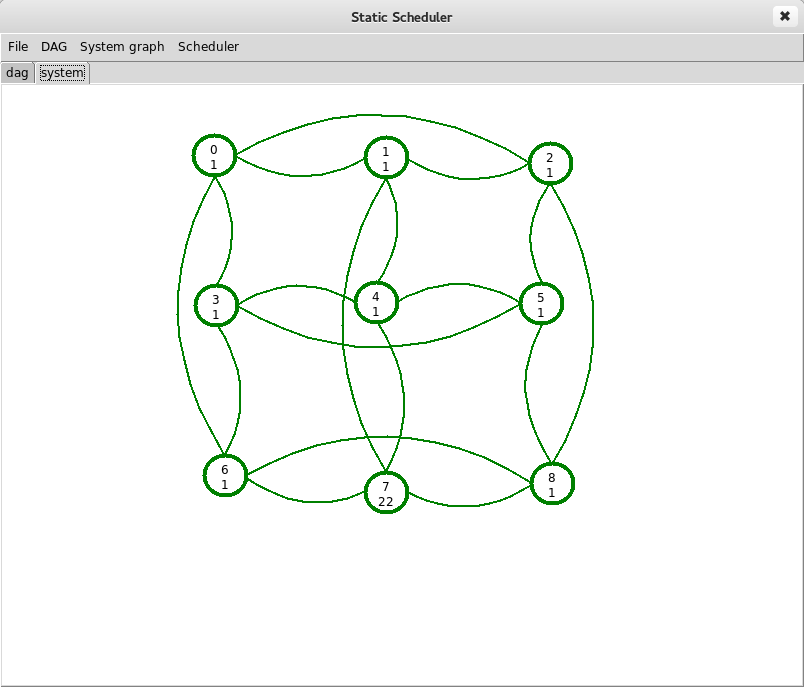
\includegraphics[width=\textwidth]{res/thor.png}
      \end{center}
      \caption{Топологія типу тор 3 порядку}
    \label{fig:thor}
    \end{figure}

    На кожному кроці зв'язності прорахуємо 15 випадкових графів та результуючий час усереднимо.
    Порахуємо коефіцієнт прискорення та коефіцієнт ефективності.

    Дуплексність присутня, процесор вводу виводу відсутній. Маштаб задачі до системи $1:1$

\begin{figure}[h]
  \begin{center}
    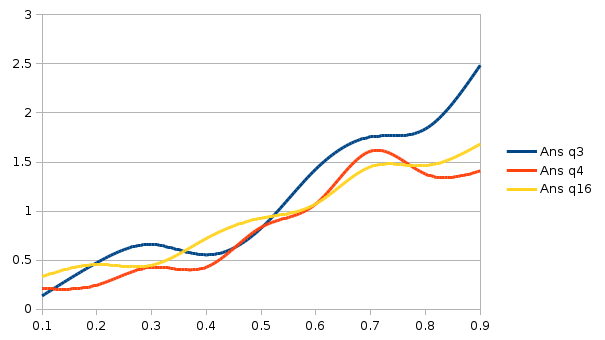
\includegraphics[width=\textwidth]{res/noio_ans.png}
  \end{center}
  \caption{Коефіцієнт прискорення алгоритму 5 без процесора вводу-виводу}
\label{fig:noio_ans}
\end{figure}

\begin{figure}[h]
  \begin{center}
    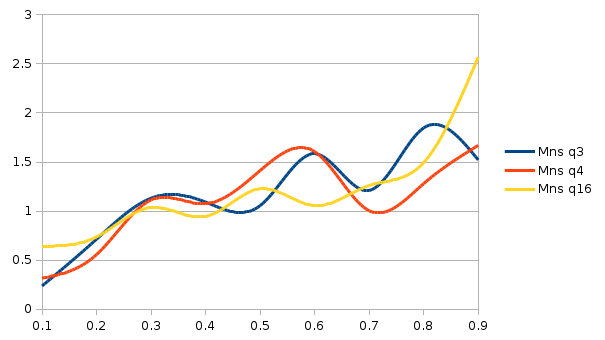
\includegraphics[width=\textwidth]{res/noio_mns.png}
  \end{center}
  \caption{Коефіцієнт прискорення алгоритму 6 без процесора вводу-виводу}
\label{fig:noio_mns}
\end{figure}

\begin{figure}[h]
  \begin{center}
    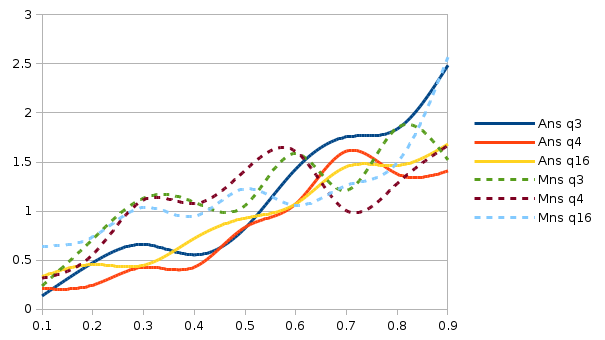
\includegraphics[width=\textwidth]{res/noio_both.png}
  \end{center}
  \caption{Суміщений графік коефіцієнтів прискорення алгоритмів 5 та 6 без процесора вводу-виводу}
\label{fig:noio_both}
\end{figure}

\begin{figure}[h]
  \begin{center}
    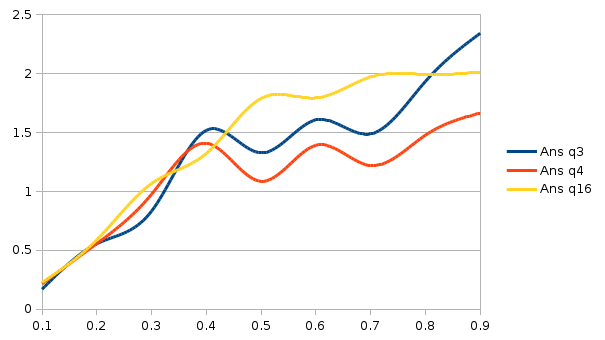
\includegraphics[width=\textwidth]{res/io_ans.png}
  \end{center}
  \caption{Коефіцієнт прискорення алгоритму 5 із процесором вводу-виводу}
\label{fig:io_ans}
\end{figure}

\begin{figure}[h]
  \begin{center}
    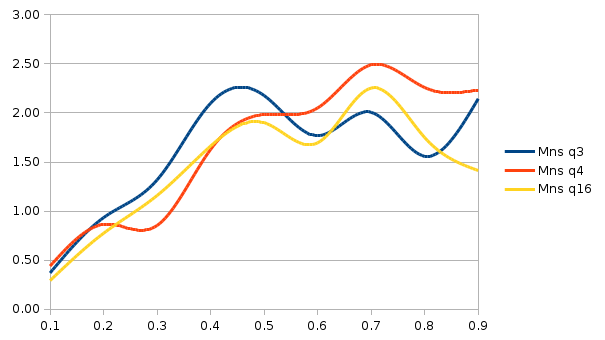
\includegraphics[width=\textwidth]{res/io_mns.png}
  \end{center}
  \caption{Коефіцієнт прискорення алгоритму 6 із процесором вводу-виводу}
\label{fig:io_mns}
\end{figure}

\begin{figure}[h]
  \begin{center}
    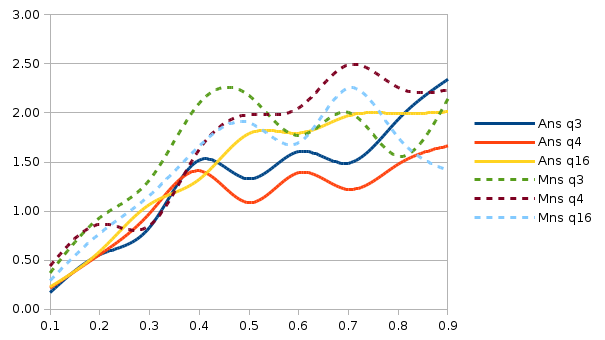
\includegraphics[width=\textwidth]{res/io_both.png}
  \end{center}
  \caption{Суміщений графік коефіцієнтів прискорення алгоритмів 5 та 6 із процесором вводу-виводу}
\label{fig:io_both}
\end{figure}


\begin{table}[H]
\caption{Алгоритм планування 5. Коефіцієнт прискорення. Процесор вводу виводу відсутній.}
\label{tab:big_table}
\centering
\begin{tabular}{lrrrrrrrrr}
\toprule
черга &   0.1 &   0.2 &   0.3 &   0.4 &   0.5 &   0.6 &   0.7 &   0.8 &   0.9 \\
\midrule
3 & 0.14 & 0.47 & 0.66 & 0.55 & 0.83 & 1.43 & 1.76 & 1.84 & 2.49 \\
4 & 0.21 & 0.25 & 0.43 & 0.43 & 0.84 & 1.07 & 1.61 & 1.38 & 1.41 \\
16 & 0.33 & 0.46 & 0.45 & 0.72 & 0.93 & 1.07 & 1.45 & 1.46 & 1.68 \\
\bottomrule
\end{tabular}
\end{table}

\begin{table}[H]
\caption{Алгоритм планування 6. Коефіцієнт прискорення. Процесор вводу виводу відсутній.}
\label{tab:big_table}
\centering
\begin{tabular}{lrrrrrrrrr}
\toprule
черга &   0.1 &   0.2 &   0.3 &   0.4 &   0.5 &   0.6 &   0.7 &   0.8 &   0.9 \\
\midrule
3 & 0.24 & 0.71 & 1.13 & 1.09 & 1.06 & 1.58 & 1.21 & 1.85 & 1.52 \\
4 & 0.32 & 0.56 & 1.11 & 1.08 & 1.41 & 1.61 & 1.00 & 1.28 & 1.67 \\
16 & 0.64 & 0.74 & 1.04 & 0.95 & 1.23 & 1.06 & 1.26 & 1.49 & 2.57 \\
\bottomrule
\end{tabular}
\end{table}


\begin{table}[H]
\caption{Алгоритм планування 5. Коефіцієнт ефективності. Процесор вводу виводу відсутній.}
\label{tab:big_table}
\centering
\begin{tabular}{lrrrrrrrrr}
\toprule
черга &   0.1 &   0.2 &   0.3 &   0.4 &   0.5 &   0.6 &   0.7 &   0.8 &   0.9 \\
\midrule
3 & 0.04 & 0.05 & 0.08 & 0.07 & 0.09 & 0.14 & 0.12 & 0.22 & 0.17 \\
4 & 0.02 & 0.03 & 0.05 & 0.05 & 0.09 & 0.12 & 0.18 & 0.15 & 0.16 \\
16 & 0.04 & 0.05 & 0.05 & 0.08 & 0.10 & 0.12 & 0.16 & 0.16 & 0.19 \\
\bottomrule
\end{tabular}
\end{table}

\begin{table}[H]
\caption{Алгоритм планування 6. Коефіцієнт ефективності. Процесор вводу виводу відсутній.}
\label{tab:big_table}
\centering
\begin{tabular}{lrrrrrrrrr}
\toprule
черга &   0.1 &   0.2 &   0.3 &   0.4 &   0.5 &   0.6 &   0.7 &   0.8 &   0.9 \\
\midrule
3 & 0.03 & 0.08 & 0.13 & 0.13 & 0.12 & 0.18 & 0.13 & 0.25 & 0.17 \\
4 & 0.04 & 0.06 & 0.12 & 0.12 & 0.16 & 0.18 & 0.11 & 0.14 & 0.19 \\
16 & 0.07 & 0.08 & 0.12 & 0.11 & 0.14 & 0.12 & 0.14 & 0.17 & 0.29 \\
\bottomrule
\end{tabular}
\end{table}

    Дуплексність присутня, процесор вводу виводу присутній. Маштаб задачі до системи $1:1$


\begin{table}[H]
\caption{Алгоритм планування 5. Коефіцієнт прискорення. Процесор вводу виводу присутній.}
\label{tab:big_table}
\centering
\begin{tabular}{lrrrrrrrrr}
\toprule
черга &   0.1 &   0.2 &   0.3 &   0.4 &   0.5 &   0.6 &   0.7 &   0.8 &   0.9 \\
\midrule
3 & 0.17 & 0.56 & 0.83 & 1.52 & 1.33 & 1.61 & 1.49 & 1.93 & 2.34 \\
4 & 0.22 & 0.56 & 0.98 & 1.41 & 1.09 & 1.39 & 1.22 & 1.48 & 1.67 \\
16 & 0.23 & 0.59 & 1.07 & 1.32 & 1.79 & 1.79 & 1.97 & 1.99 & 2.01 \\
\bottomrule
\end{tabular}
\end{table}

\begin{table}[H]
\caption{Алгоритм планування 6. Коефіцієнт прискорення. Процесор вводу виводу присутній.}
\label{tab:big_table}
\centering
\begin{tabular}{lrrrrrrrrr}
\toprule
черга &   0.1 &   0.2 &   0.3 &   0.4 &   0.5 &   0.6 &   0.7 &   0.8 &   0.9 \\
\midrule
3 & 0.37 & 0.73 & 1.02 & 2.10 & 2.18 & 1.77 & 2.01 & 1.56 & 2.14 \\
4 & 0.44 & 0.86 & 0.85 & 1.93 & 1.38 & 2.55 & 2.49 & 2.26 & 1.93 \\
16 & 0.29 & 0.77 & 1.16 & 1.66 & 1.90 & 1.70 & 2.25 & 1.75 & 1.41 \\
\bottomrule
\end{tabular}
\end{table}

\begin{table}[H]
\caption{Алгоритм планування 5. Коефіцієнт ефективності. Процесор вводу виводу присутній.}
\label{tab:big_table}
\centering
\begin{tabular}{lrrrrrrrrr}
\toprule
черга &   0.1 &   0.2 &   0.3 &   0.4 &   0.5 &   0.6 &   0.7 &   0.8 &   0.9 \\
\midrule
3 & 0.02 & 0.06 & 0.09 & 0.17 & 0.15 & 0.18 & 0.17 & 0.21 & 0.26 \\
4 & 0.02 & 0.06 & 0.11 & 0.16 & 0.12 & 0.15 & 0.14 & 0.16 & 0.19 \\
16 & 0.03 & 0.07 & 0.12 & 0.15 & 0.20 & 0.20 & 0.22 & 0.22 & 0.22 \\
\bottomrule
\end{tabular}
\end{table}

\begin{table}[H]
\caption{Алгоритм планування 6. Коефіцієнт ефективності. Процесор вводу виводу присутній.}
\label{tab:big_table}
\centering
\begin{tabular}{lrrrrrrrrr}
\toprule
черга &   0.1 &   0.2 &   0.3 &   0.4 &   0.5 &   0.6 &   0.7 &   0.8 &   0.9 \\
\midrule
3 & 0.04 & 0.08 & 0.11 & 0.23 & 0.24 & 0.20 & 0.22 & 0.17 & 0.24 \\
4 & 0.05 & 0.10 & 0.09 & 0.21 & 0.15 & 0.28 & 0.28 & 0.25 & 0.21 \\
16 & 0.03 & 0.09 & 0.13 & 0.18 & 0.21 & 0.19 & 0.25 & 0.19 & 0.16 \\
\bottomrule
\end{tabular}
\end{table}

Як можна сказати з графіку \ref{fig:noio_both} при відсутності процесору вводу/виводу приблизно до зв'язності 0.6 найбільш ефективними є алгоритми з моделюванням. На ділянці 0.1-0.6 правильним вибором буде алгоритм 6 із 4 алгоритмом черги.

Після 0.6 немає чіткої різниці між алгоритмами. Тому, зважаючи на вимірювання часу із наступного розділу, при зв'язності більшій ніж 0.6 рекомендовано використовувати алгоритм 5 сусіднього призначення із чергою 3, як найбільш ефективного по часу та дещо більшого за коефіцієнтом прискорення за інші алгоритми.

З графіку \ref{fig:io_both} при наявності процесору вводу/виводу аналіз дає дещо інші результати. На всій ділянці від 0.1 до 0.9 найбільш ефективними є алгоритми 6 з моделюванням. При цьому на проміжку 0.1-0.5 це алгоритм 6 з чергою 3, а на проміжку 0.6-0.9 це алгоритм 6 з чергою 4.

Судячи з графіків, варіант із процесорами вводу-виводу є більш ефективним. Для подальшого аналізу оберемо систему із процесорами вводу/виводу, і проаналізуємо роботу алгоритмів 6-3 та 6-4 на проміжках 0.1-0.5 та 0.6-0.9 відповідно на іншій топології та з іншими параметрами системи.

\subsection{Порівняння часу роботи алгоритмів планування}

Для порівняння часу роботи 5 та 6 алгоритмів зробимо замір часу для кожної зв'язності від 0.1 до 0.9 при увімкненому дуплексі та процесорах вводу/виводу.
Необхідності перевіряти час роботи на всіх алгоритмах формування черги немає, тому що вони еквівалентні за складністю та не внесуть змін у статистику.

\begin{table}[H]
\caption{Час роботи алгоритмів (msec)}
\label{tab:big_table}
\centering
\begin{tabular}{llrrrrrrrrr}
\toprule
Алгоритм & Черга &   0.1 &   0.2 &   0.3 &   0.4 &   0.5 &   0.6 &   0.7 &   0.8 &   0.9 \\
\midrule
5 & 3 & 391 & 320 & 299 & 280 & 264 & 258 & 251 & 251 & 252 \\
6 & 3 & 513 & 387 & 340 & 326 & 312 & 302 & 299 & 298 & 295 \\
\bottomrule
\end{tabular}
\end{table}

\subsection{Вивчення впливу топології}

Для порівняння результатів візьмемо схожу на тор топологію - решітка 3 порядку (рис. \ref{fig:grid}).

    \begin{figure}[h!]
      \begin{center}
        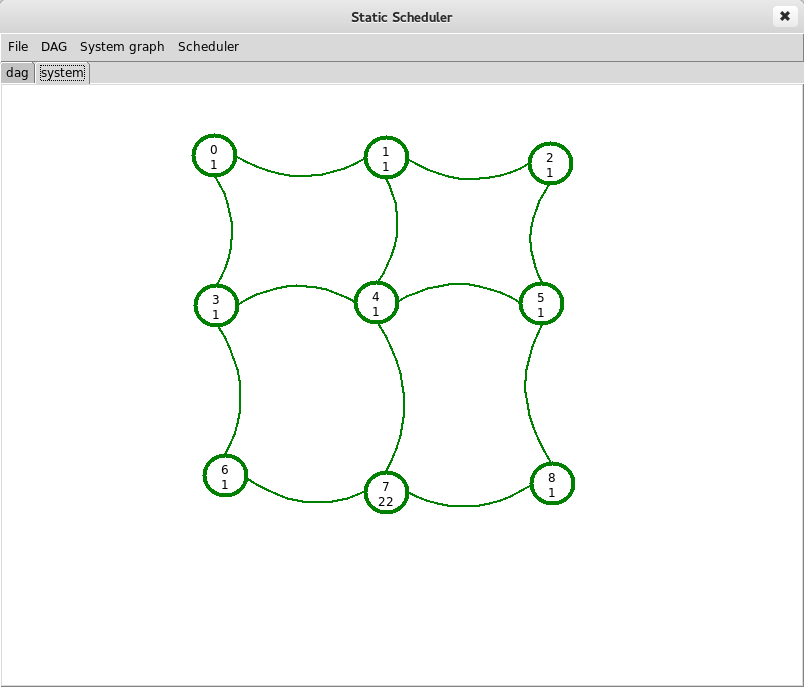
\includegraphics[width=\textwidth]{res/grid.png}
      \end{center}
      \caption{Топологія типу решітка 3 порядку}
    \label{fig:grid}
    \end{figure}
